\begin{table*}[t]%
    \begin{DndTable}[width=\linewidth]{X}
        \centering
        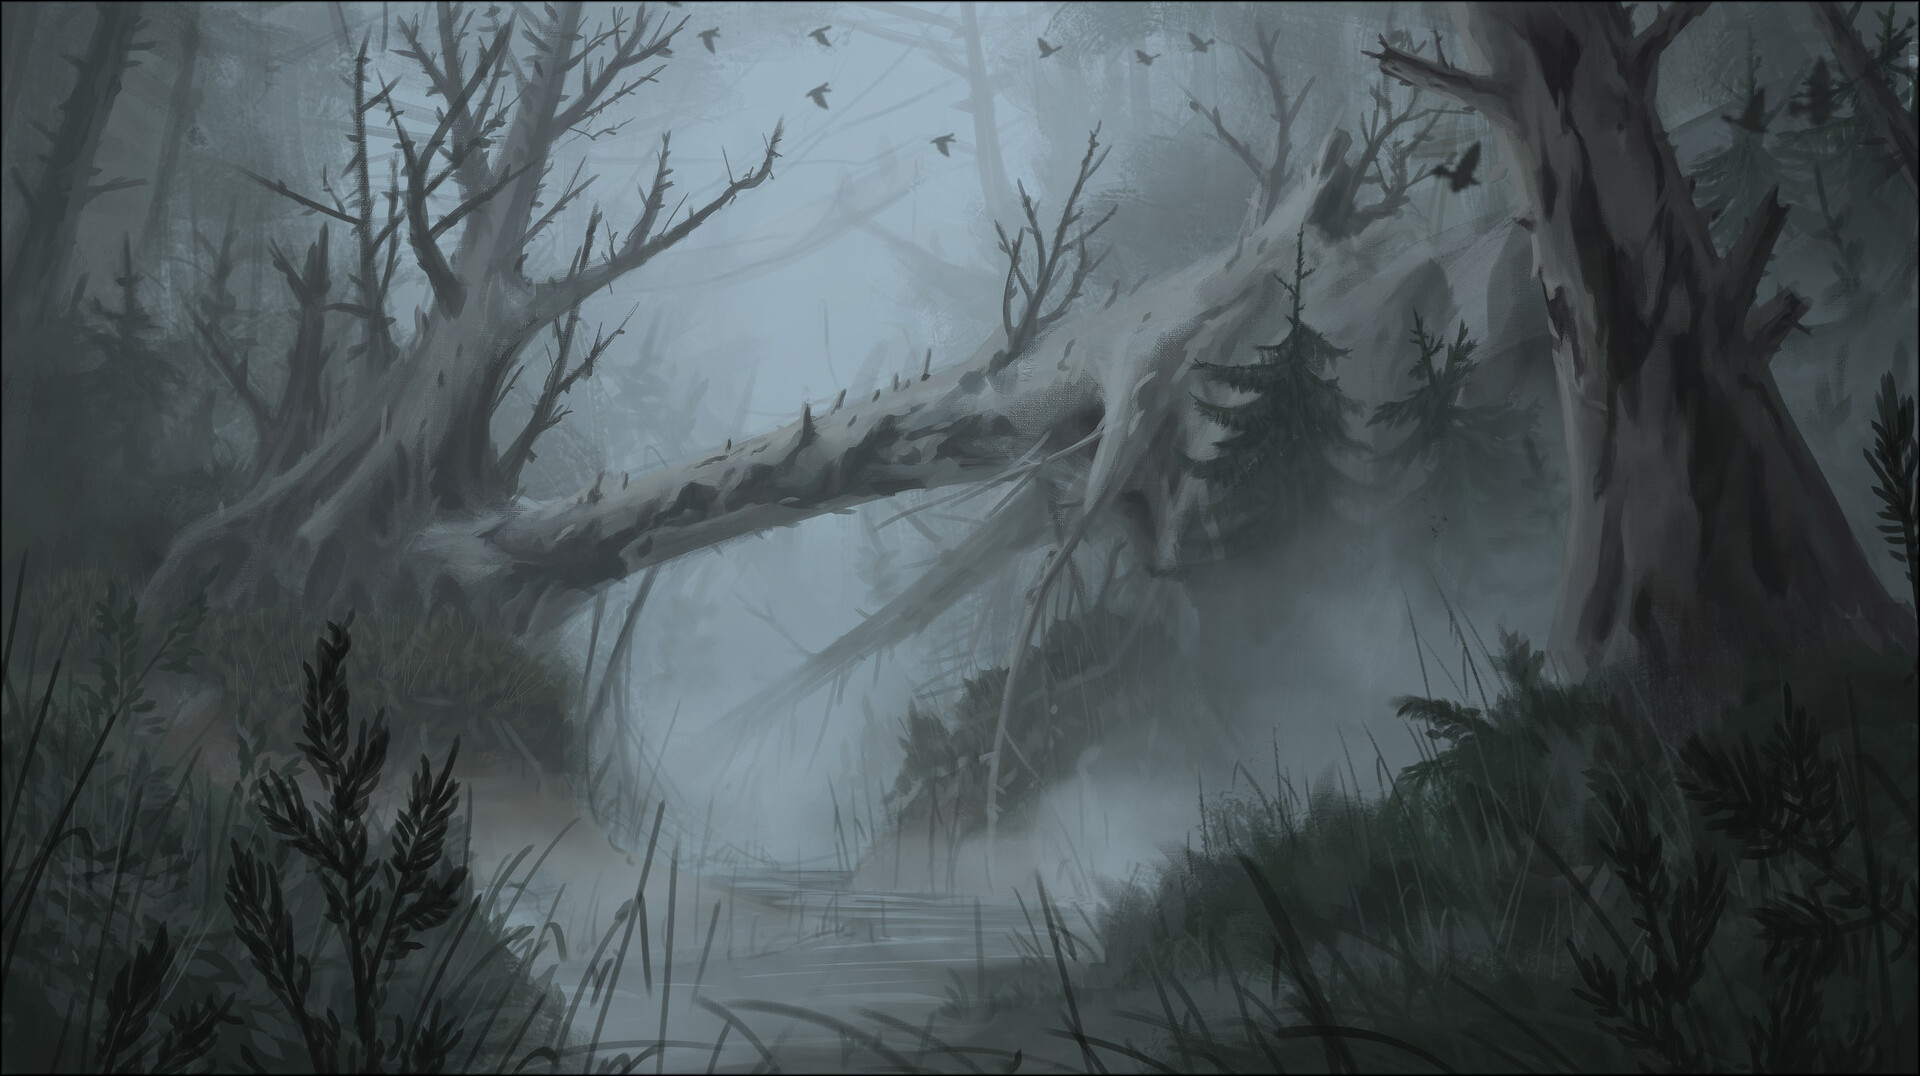
\includegraphics[width=0.98\textwidth]{01intro/img/16pale_blemish.png} \
        \centering \large{\textbf{Forests Surrounding the Pale Blemish}}
    \end{DndTable}
\end{table*}

\subsection*{Wildlands}
% intro
The southernmost region of Yuadrem is aptly named the Wildlands, for it is a large expanse of untamed fields, forests, and lakes.
Starting at the bottom-most part of the forking peaks, the area has seen very little intervention from the civilized world.
This is attributed to the fact that the Wildlands are infested with both deadly creatures and strange tide-altering illnesses.

% Savage Plains
Just below the forking peaks and the Beal river is the northmost point of the Wildlands, the Savage Plains.
They are a humid subtropical area covered by marshes and plains, with few patches of forest in-between.
Fed by many rivers from the mountains, the lands define the southern territories of the Iskenese empire, expanding thorough the whole region.

However, Isken's grip on the Savage Plains is tenuous at best, as the region is as much controlled by the grungs as it is by the local wildlife.
Just as in the forest below, a great variety of foul beasts and creatures can be found in these swamps.
Of special note among these are the giant mole-like jinshus, beasts unique to region who suffocate the unprepared by sinking them beneath the earth.

% Everwoods
As dangerous as these plains are the Everwoods, the forest that grows south of them.
This ancient woodland used to be a place of respite after the harsh swamps, but all that swiftly changed about 400 years ago.
In an attempt to manipulate the tides, the Rashiist school of thought from Ignelli summoned The Sorrow into Yuadrem.
The Sorrow is an entity of unknown origin, who seeped into Yuadrem due to the Rashiists folly.
On arrival, it swiftly slayed all members of the school of thought, and brought fourth with it strange creatures and diseases that now plague the once peaceful forest.
This event came to be known as the Tidal Sway.

% Pale Blemish
Not only bringing forth pain and disease, the Tidal Sway also ravaged the land around Ignelli, area now known as the pale blemish.
All flora was destroyed, and the ground turned into badlands.
The field now serves as a grim reminder to all of the dangers of manipulating the tides.

Despite the destruction, the scholars from the Igneist school continue to work in their temple, studying the tides and The Sorrow.
Perhaps one day they'll achieve their goal and undo their sister school's sins, expelling the Sorrow and healing their lands.

% Niknek Peninsula
West of the Everwoods is the Niknek peninsula, a thin, elongated stretch of land filled with volcanoes and gorges.
The cape was spared from most of the effects of the Tidal Sway.
Niknek and the nearby Vuvu Isles now house the refuge marsets from the Springwater Island.

% Elderberry Wilds
At the southern tip of Yuadrem are the Elderberry Wilds and the Ironwoods, a set of pine and spruce forest surrounding the Manta Sea.
The area is partly occupied by Gronselar, an old and forgotten colony of Krudzal.
% Not much is known about these forests due to their remote location.
% Not much is known about the area due to its remote location, but even here a semblance of civilization exists. in the form of the ird nation of Gronselar, and the regions of Froibias, Glameas, and Visilias.
